\documentclass[11pt]{article}

% Change "review" to "final" to generate the final (sometimes called camera-ready) version.
% Change to "preprint" to generate a non-anonymous version with page numbers.
\usepackage[preprint]{acl}

% Standard package includes
\usepackage{times}
% times maps \tt to Courier (pcr); Basic TeX often lacks Courier metrics (pcrr8t).
% Keep roman/sansserif from the PSNFSS bundle but use Computer Modern typewriter.
\renewcommand{\ttdefault}{cmtt}
\usepackage{latexsym}

% For proper rendering and hyphenation of words containing Latin characters (including in bib files)
\usepackage[T1]{fontenc}
% For Vietnamese characters
% \usepackage[T5]{fontenc}
% See https://www.latex-project.org/help/documentation/encguide.pdf for other character sets

% This assumes your files are encoded as UTF8
\usepackage[utf8]{inputenc}

% This is not strictly necessary, and may be commented out,
% but it will improve the layout of the manuscript,
% and will typically save some space.
\usepackage{microtype}

% This is also not strictly necessary, and may be commented out.
% However, it will improve the aesthetics of text in
% the typewriter font. Optional: TeX Live Basic omits inconsolata; install with
% `tlmgr install inconsolata` (or use MacTeX/full TeX Live). If the .sty is
% missing, we skip loading—avoid substituting courier.sty alone, which can fail
% when the matching TFM fonts are not installed.
\IfFileExists{inconsolata.sty}{%
  \usepackage{inconsolata}%
}{}

%Including images in your LaTeX document requires adding
%additional package(s)
\usepackage{graphicx}

% algorithms/tikz are not in TeX Live Basic; omit if missing (fine for text-only papers).
\IfFileExists{algorithm.sty}{%
  \usepackage{algorithm}%
  \usepackage{algpseudocode}%
}{}
\usepackage{amsmath}
\usepackage{booktabs}

% TikZ required for figures in \texttt{final.tex} (DP denoising diagram).
\usepackage{tikz}
\usetikzlibrary{positioning,arrows.meta,calc,fit,backgrounds,decorations.pathreplacing}
\usepackage{xcolor}
% If the title and author information does not fit in the area allocated, uncomment the following
%
%\setlength\titlebox{<dim>}
%
% and set <dim> to something 5cm or larger.

% \title{ANLP Final Project}
\title{Dgrammar and DPGrammar: Frontier Constrained Decoding for Diffusion Language Models}


\author{
    \textbf{Jeng-Yue Liu\textsuperscript{1}},
    \textbf{Wilson Zheng\textsuperscript{1}},
    \textbf{Haoling Pu\textsuperscript{1}}
    \\
    \textsuperscript{1}Language Technologies Institute, Carnegie Mellon University
    \\
    \texttt{\{buffettl,wilsonz,haolingp\}@andrew.cmu.edu}
} 


\begin{document}
\maketitle
% % Requirement
% Motivation
% What is the general research topic?
% What is the significance of the research topic? Why is this topic worth working on?
% Literature Review
% Provide a broad view of the relevant research landscape
% Provide concrete descriptions on a small handful of the most highly related works.
% Identify major trends/patterns across prior work.
% Identify shortcomings with prior work and/or other opportunities that motivate this work
% Initial Proposed Approaches
% Provide high-level descriptions for at least 2 potential approaches to innovate on the research topic
% see "Suggestions for Brainstorming Project Ideas" below for concrete advice
% be sure to consider compute requirements, and provide an estimate in your report
% Initial Proposed Data
% Identify data sources that will be useful for training (if applicable) and evaluation.
% Initial Proposed Evaluation
% Which concepts or theoretical constructs are most relevant for evaluating your method, and why?
% If the constructs can’t be directly measured, what metrics will serve as acceptable proxies?
% If your system consists of multiple components, what constructs/metrics will you use to evaluate the sub-components?
% What qualitative analyses do you plan to conduct?



% \begin{abstract}
% Abstract here
% \end{abstract}

\section{Motivation} % Introduction

% 1. Structure decoding importance
% The difference in diffusion and AR structure decoding
% why it worth research for structure decoding in diffusion
% Current downside
% constrained decoding + LAVE
% their downside O(N) pick candidates
% solve: CSR matrix + Herding algorithm

% 2. Deterministic > probabilistic
% sampling wall causing information collapse

Diffusion large language models (dLLMs) have emerged as a promising alternative to autoregressive (AR) models, offering parallel token generation and bidirectional context modeling. A critical challenge in deploying dLLMs for structured generation tasks, as shown in figure \ref{fig:constraint-pass-fail}, such as JSON schema compliance, code synthesis, and chemical expression generation, is ensuring that outputs reliably conform to formal grammar constraints \citep{cd4dllm}.

\begin{figure*}[t]
\centering
\resizebox{\textwidth}{!}{%
    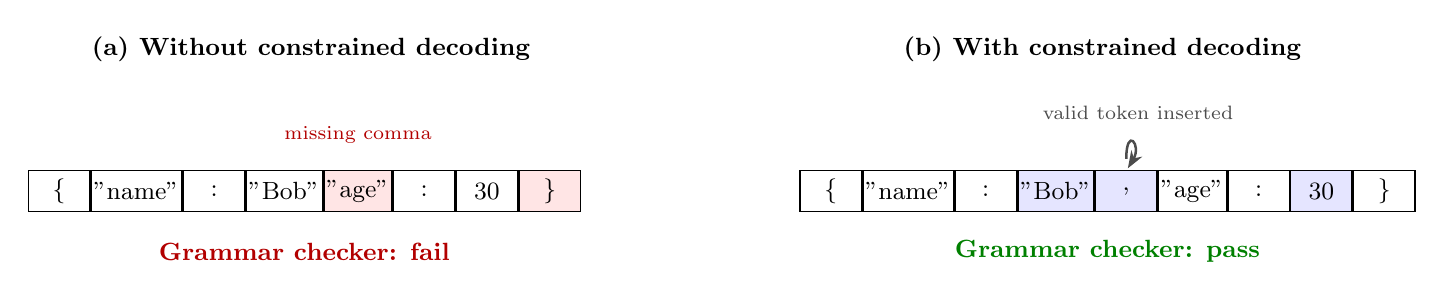
\begin{tikzpicture}[
        font=\small,
        tok/.style={
            draw=black,
            line width=0.5pt,
            minimum width=0.78cm,
            minimum height=0.52cm,
            align=center,
            inner sep=1pt
        },
        good/.style={
            tok,
            fill=blue!10
        },
        bad/.style={
            tok,
            fill=red!10
        },
        title/.style={
            font=\small\bfseries
        },
        noteok/.style={
            font=\small\bfseries,
            text=green!50!black
        },
        notebad/.style={
            font=\small\bfseries,
            text=red!70!black
        },
        smallnote/.style={
            font=\scriptsize
        },
        arr/.style={
            -{Stealth[length=2.2mm,width=1.6mm]},
            line width=0.9pt,
            draw=black!70
        }
    ]
    
    % =========================
    % Left panel
    % =========================
    \node[title] at (3.2,1.8) {(a) Without constrained decoding};
    
    \node[tok] (L1) at (0,0) {\{};
    \node[tok, right=0cm of L1] (L2) {"name"};
    \node[tok, right=0cm of L2] (L3) {:};
    \node[tok, right=0cm of L3] (L4) {"Bob"};
    \node[bad, right=0cm of L4] (L5) {"age"};
    \node[tok, right=0cm of L5] (L6) {:};
    \node[tok, right=0cm of L6] (L7) {30};
    \node[bad, right=0cm of L7] (L8) {\}};
    
    \node[smallnote, text=red!70!black] at ($(L5.north)+(0,0.45)$) {missing comma};
    
    \node[notebad] at ($(L1.south)!0.5!(L8.south)+(0,-0.5)$) {Grammar checker: fail};
    
    % =========================
    % Right panel
    % =========================
    \begin{scope}[xshift=9.8cm]
    
    \node[title] at (3.45,1.8) {(b) With constrained decoding};
    
    \node[tok] (R1) at (0,0) {\{};
    \node[tok, right=0cm of R1] (R2) {"name"};
    \node[tok, right=0cm of R2] (R3) {:};
    \node[good, right=0cm of R3] (R4) {"Bob"};
    \node[good, right=0cm of R4] (R5) {,};
    \node[tok, right=0cm of R5] (R6) {"age"};
    \node[tok, right=0cm of R6] (R7) {:};
    \node[good, right=0cm of R7] (R8) {30};
    \node[tok, right=0cm of R8] (R9) {\}};
    
    \draw[arr] ($(R5.north)+(0,0.14)$)
        .. controls +(0,0.42) and +(0.18,0.30) ..
        ($(R5.north)+(0.02,0.02)$);
    
    \node[smallnote, text=black!70] at ($(R5.north)+(0.15,0.72)$) {valid token inserted};
    
    \node[noteok] at ($(R1.south)!0.5!(R9.south)+(0,-0.5)$) {Grammar checker: pass};
    
    \end{scope}
    
    \end{tikzpicture}%
}
\caption{
Example of unconstrained versus grammar-constrained decoding.
Without constraints, the model may emit an invalid continuation, causing the grammar check to fail.
With constrained decoding, invalid continuations are pruned during generation, yielding a grammar-valid output.
}
\label{fig:constraint-pass-fail}
\end{figure*}


The state-of-the-art approach, LAVE \citep{zhang2026lookaheadthenverifyreliableconstraineddecoding}, addresses this by leveraging dLLMs' ability to predict token distributions for all positions in parallel during each forward pass. When the model proposes a token, LAVE performs lookahead by sampling $N$ complete prefixes for the remaining masked positions and accepts the token only if at least one sampled prefix passes a grammar parser. While effective, this approach has two fundamental limitations.

First, the verification process in LAVE is inherently stochastic. Because it relies on random sampling to fill masked positions, there is a persistent, non-zero probability that a valid token will be erroneously rejected. This occurs when none of the $N$ generated samples yield a parseable prefix, triggering unnecessary retries and degraded generation quality.

Second, LAVE evaluates token decisions independently at each position, mirroring the left-to-right bottlenecks of AR models. When multiple positions are unmasked during a single diffusion step, LAVE verifies each token in isolation, ignoring the joint dependencies between simultaneously unmasked slots. Thus, while individual tokens may pass local verification, their combination can create a dead-end for subsequent tokens, rendering them illegal. This greedy, position-by-position strategy is fundamentally misaligned with the parallel nature of diffusion generation.

We propose Grammar-Guided Beam Search (GGBS), a deterministic constrained decoding framework that integrates structural constraints directly into the beam expansion process. By replacing post-hoc random sampling with incremental parser state tracking, GGBS eliminates the stochastic rejection of valid tokens; instead, it performs a deterministic top-$K$ selection from a set of grammar-valid candidates. Crucially, GGBS shifts the decoding paradigm from independent token validation to a joint optimization over all masked positions within a diffusion step. By maintaining parser states across both fixed and masked segments, GGBS identifies the highest-probability token assignment that satisfies global grammar constraints across the entire unmasked span. This approach aligns the decoding process with the parallel nature of diffusion, ensuring structural coherence without the efficiency trade-offs of greedy, position-by-position verification. The code is available at github \url{https://github.com/buffett0323/anlp_final}.


% While discrete diffusion language models (dLLMs) offer a parallelized alternative to autoregressive (AR) generation, our analysis identifies a Trilemma of Inefficiency that prevents their deployment in production-scale structured decoding.

% First, the system is hindered by \textbf{search width}, where enforcing constraints requires an exhaustive $O(V)$ scan of the entire vocabulary to identify valid transitions at every step. Existing constrained diffusion frameworks, such as DINGO \citep{suresh2025dingoconstrainedinferencediffusion}, require an exhaustive scan over the full vocabulary $V$ to identify valid transitions at every denoising step. This linear dependence on vocabulary size introduces substantial memory and I/O overhead on modern accelerators, undermining the throughput advantage of non-autoregressive generation.

% Second, it also suffers from a lack of \textbf{information integrity} due to the ``sampling wall,'' a phenomenon where rich probability distributions are discarded in favor of sparse one-hot token commitments \citep{jo2026loopholingdiscretediffusiondeterministic}. Standard dLLMs rely on stochastic ancestral sampling, in which rich token distributions are collapsed into one-hot commitments at each step. In structured generation, a high-probability token may be temporarily disallowed by a grammar constraint (e.g., a required JSON bracket). Once suppressed, that latent preference can be lost, causing the model to forget its original semantic intent and increasing the risk of logical dead-ends.

% Third, the \textbf{inference depth} remains a bottleneck, as standard unmasking schedules require a high number of function evaluations (NFE)\footnote{NFE is the number of times the model must perform a forward denoising step during inference to produce an output.} to maintain syntactic accuracy, often nullifying the theoretical latency benefits inherent to the diffusion paradigm. High-quality structured generation often requires a large NFE. Although speculative decoding has become an effective acceleration technique for AR models \citep{leviathan2023fastinferencetransformersspeculative}, dLLMs still lack a mechanism for verifying multiple future structural positions within a single forward pass while preserving strict syntactic correctness.

% To address these barriers, we propose the \textbf{Sparse Deterministic Speculative Decoding (SD2)} framework. SD2 combines three key ideas: (i) flattening formal automata into CSR matrices for effectively $O(1)$ vectorized token retrieval; (ii) replacing stochastic sampling with a deterministic herding algorithm that preserves token momentum across denoising steps; and (iii) introducing grammar-legal speculative trees that exploit the bidirectional context of dLLMs to accelerate convergence. By combining hardware-native indexing, deterministic intent preservation, and structure-aware speculation, SD2 provides a scalable pathway for deploying strictly constrained diffusion engines in latency-sensitive environments.


% -----

% While discrete diffusion language models (dLLMs) offer a parallelized alternative to autoregressive (AR) generation, our analysis shows that the current state of the art still faces three critical barriers to production-scale structured decoding. First, the system is hindered by \textbf{Search Width}, where enforcing constraints requires an exhaustive $O(N)$ scan of the entire vocabulary to identify valid transitions at every step. Second, it suffers from a lack of \textbf{Information Integrity} due to the ``sampling wall,'' a phenomenon where rich probability distributions are discarded in favor of sparse one-hot token commitments. Finally, the \textbf{Inference Depth} remains a bottleneck, as standard unmasking schedules require a high number of function evaluations (NFE) to maintain syntactic accuracy, often nullifying the theoretical latency benefits inherent to the diffusion paradigm.

% To address these challenges, existing works have proposed mathematically rigorous but computationally expensive solutions. DINGO \citep{suresh2025dingoconstrainedinferencediffusion} successfully introduced the first provably correct dynamic programming (DP) framework for dLLMs to ensure 100\% syntactic correctness. However, its transition cost calculation iterates through the full vocabulary $V$, resulting in a complexity of $O(d \cdot |Q| \cdot |V|)$ per block. This linear dependence on vocabulary size creates a significant I/O overhead on modern accelerators. Furthermore, the reliance on stochastic ancestral sampling leads to a ``sampling wall'' \citep{jo2026loopholingdiscretediffusiondeterministic}, where the soft information about alternative token candidates collapses into a single category. In structured tasks, where high-probability tokens are often suppressed by temporary grammar constraints (e.g., a required JSON bracket), this collapse prevents the model from remembering its original intent, leading to oscillations or logical dead-ends. While recent paradigms like LAVE \citep{zhang2026lookaheadthenverifyreliableconstraineddecoding} and Plan-Verify-Fill (PVF) \citep{li2026planverifyfillstructured} attempt to improve reliability through lookahead or structural anchors, they primarily serve as statistical filters and do not resolve the underlying $O(N)$ retrieval complexity or the serial nature of step-by-step unmasking.

% We propose the Sparse Deterministic Speculative Decoding (SD2) framework to systematically overcome these three dimensions of inefficiency. To optimize the search width, we incorporate the STATIC framework \citep{su2026vectorizingtrieefficientconstrained} to flatten formal automata into hardware-friendly Compressed Sparse Row (CSR) matrices, recasting token retrieval as vectorized $O(1)$ memory access through coalesced reads. To ensure information integrity, we replace stochastic sampling with a deterministic Herding algorithm \citep{herding}, maintaining a continuous weight vector that preserves the momentum of suppressed tokens across denoising steps, allowing blocked intents to resurface once the grammar state permits \citep{suzuki2026deterministicdiscretedenoising}. Finally, we address inference depth by constructing grammar-legal speculative trees, leveraging the inherent bidirectional context of dLLMs to verify multiple future structural positions in a single forward pass. By synergizing sub-linear sparse indexing with deterministic intent preservation, SD2 provides a scalable pathway for deploying strictly constrained diffusion engines in real-world, latency-sensitive environments such as automated programming and symbolic reasoning. The code is available at github \url{https://github.com/buffett0323/SD2}.



\section{Literature Review}

\subsection{Discrete Diffusion and Parallel Decoding}
Discrete diffusion models (dLLMs) such as LLaDA \citep{llada} and Dream \citep{dream} represent a paradigm shift from traditional AR models by enabling non-autoregressive, any-order text generation through iterative refinement. However, this flexibility introduces the incomplete prefix problem: unlike AR models, where a stable prefix always exists for grammar state tracking, dLLMs must often predict tokens surrounded by unmasked or partially denoised noise. While recent acceleration techniques like DFlash \citep{chen2026dflashblockdiffusionflash} and Spiffy \citep{agrawal2026spiffymultiplyingdiffusionllm} reduce the sampling steps via block-diffusion, they remain ``unconstrained,'' failing to guarantee structural or syntactic correctness in the generated output.

\subsection{Constrained Decoding: From AR to dLLMs}
Traditional constrained decoding frameworks like \textit{Outlines} \citep{outlines} and \textit{XGrammar} \citep{dong2024xgrammar} rely on the linear progression of AR decoding to maintain finite state machine (FSM) or parser states. These methods cannot be directly applied to dLLMs due to the lack of a monotonic causal chain. 
Transitioning these constraints to the diffusion paradigm, \citet{cd4dllm} proposed the first Context-Free Grammer (CFG-constrained) dLLM decoder, while DINGO \citep{suresh2025dingoconstrainedinferencediffusion} utilized dynamic programming (DP) to ensure syntactic correctness, albeit at a high computational cost. LAVE \citep{zhang2026lookaheadthenverifyreliableconstraineddecoding} introduced a ``lookahead-then-verify'' mechanism as a baseline for reliability; however, LAVE's reliance on stochastic sampling for verification possibly lead to the rejection of valid tokens. Our work draws inspiration from the STATIC framework \citep{su2026vectorizingtrieefficientconstrained}, which demonstrated that sparse transition structures can be flattened into Compressed Sparse Row (CSR) matrices to enable $O(K)$ coalesced lookups, where $K$ is the branch factor, rather than scanning the full vocabulary of size $|V|$. We adapt this principle to represent DFA token-level transitions for grammar-constrained decoding, reducing the per-step transition cost in our bidirectional Viterbi DP from $O(|V|)$ to $O(K)$.


% \subsection{Deterministic Dynamics in Discrete Spaces}
% A significant challenge in discrete diffusion is the "sampling wall"—the information loss occurring when categorical distributions are discretized via random sampling. Research into Deterministic Discrete Denoising \citep{suzuki2026deterministicdiscretedenoising} and the Herding algorithm \citep{herding} suggests that replacing stochastic sampling with deterministic state transitions can preserve the "working memory" of suppressed tokens. By adopting deterministic dynamics, our proposed GGBS eliminates the "luck-of-the-draw" failure modes found in LAVE, ensuring that the highest-probability grammar-valid paths are consistently selected rather than sampled.

\subsection{Beam Search and Joint Multi-Token Decoding}
While classic beam search is a staple of AR decoding, its application in dLLMs requires a fundamental shift toward joint optimization. In diffusion steps where multiple positions are unmasked simultaneously, independent token-wise verification fails to account for inter-token dependencies, often leading to globally invalid sequences. \citet{leviathan2023fastinferencetransformersspeculative} has demonstrated the power of parallel verification in AR contexts; however, existing dLLM methods often revert to greedy, position-by-position checks. GGBS addresses this by treating the unmasked span as a joint decoding problem, utilizing bidirectional suffix feasibility pruning to ensure that the chosen tokens satisfy grammar constraints globally rather than just locally.


% \section{Literature Review}

% \subsection{Discrete Diffusion and Parallel Decoding}
% Discrete diffusion models like LLaDA-8B \citep{llada} and Dream-7B \citep{dream} generate text through iterative refinement, breaking the strict causal constraints of AR models. While they enable any-order generation, their practical utility is often limited by high NFE requirements. Recent efforts like DFlash \citep{chen2026dflashblockdiffusionflash} and Spiffy \citep{agrawal2026spiffymultiplyingdiffusionllm} attempt to reduce this overhead via block-diffusion or self-speculative mechanisms, yet these acceleration techniques have not been natively integrated with formal structural constraints.

% \subsection{Formal Constraints in dLLMs}
% The transition from statistical generation to symbolic accuracy has led to frameworks like DINGO \citep{suresh2025dingoconstrainedinferencediffusion}, which employs dynamic programming (DP) to ensure 100\% syntactic correctness in diffusion. However, the computational cost of DP in dLLMs remains high. While LAVE \citep{zhang2026lookaheadthenverifyreliableconstraineddecoding} and PVF \citep{li2026planverifyfillstructured} improve reliability through lookahead or planning strategies, they function primarily as high-level filters. Our work builds upon the STATIC framework \citep{su2026vectorizingtrieefficientconstrained}, which demonstrated that flattening trie-based constraints into Compressed Sparse Row (CSR) matrices can transform irregular memory access into hardware-friendly vectorized operations, offering a path to bypass the $O(|V|)$ retrieval bottleneck.

% \subsection{Deterministic Dynamics and Intent Preservation}
% A core challenge in discrete state spaces is the ``sampling wall'', the information loss occurring when categorical distributions are discretized. Research into Deterministic Discrete Denoising \citep{suzuki2026deterministicdiscretedenoising} suggests that transforming stochastic sampling into deterministic state transitions can maintain a ``working memory'' of suppressed tokens. This approach, rooted in the Herding algorithm, allows models to achieve faster asymptotic convergence. SD2 integrates these deterministic dynamics specifically to solve the intent-grammar mismatch often found in structured decoding.

% \subsection{Speculative Tree Verification}
% Speculative decoding has successfully accelerated AR models by using draft models to propose multiple tokens for parallel verification \citep{leviathan2023fastinferencetransformersspeculative}. In the diffusion paradigm, SSD leverages the model’s inherent parallel prediction capability. However, existing speculative methods for diffusion often revert to expensive pointer-chasing structures for constraint enforcement. SD2 extends this by constructing speculative trees that are inherently grammar-legal, utilizing the bidirectional nature of dLLMs to verify structural anchors across multiple positions simultaneously.


% \subsection{Discrete Diffusion Language Models}
% Discrete diffusion models have emerged as a significant alternative to AR architectures, enabling text generation through iterative refinement in discrete state spaces. Unlike AR models that are bound by strict causal factorization, models such as LLaDA-8B \citep{llada} and Dream-7B \citep{dream} utilize bidirectional attention to decode token blocks in parallel, offering superior flexibility for any-order generation and infilling. Despite their parallel potential, these models often require a high NFE to match the quality of AR counterparts, motivating the need for more efficient unmasking and remasking strategies.

% \subsection{Constrained Inference in Non-Autoregressive Paradigms}
% Enforcing structural correctness in probabilistic generators has traditionally relied on finite-state machines (FSM) or pushdown automata (PDA) to mask logits during sequential decoding, as seen in libraries like Outlines \citep{outlines} and XGrammar \citep{dong2024xgrammar}. DINGO \citep{suresh2025dingoconstrainedinferencediffusion} represents the first provably correct constrained decoding framework for diffusion LLMs, employing DP to find the highest-probability path that satisfies regular expression constraints. However, DINGO’s search process scales with the full vocabulary size $N$, incurring significant runtime overhead. More recently, LAVE \citep{li2026planverifyfillstructured} introduced a "lookahead-then-verify" mechanism to improve reliability for context-free grammars (CFG), yet it primarily serves as a statistical filter without addressing the underlying computational complexity of token retrieval.


% \subsection{Deterministic Dynamics and the Sampling Wall}
% A fundamental limitation of discrete diffusion is the ``sampling wall,'' where rich categorical distributions collapse into sparse one-hot vectors, leading to information loss across denoising steps. \citet{suzuki2026deterministicdiscretedenoising} proposed Deterministic Discrete Denoising based on the herding algorithm, which transforms stochastic sampling into deterministic state transitions governed by continuous weight vectors. This mechanism effectively maintains a working memory of suppressed token momentum, allowing for faster asymptotic convergence ($O(T^{-1})$) and higher sample quality. Recent paradigms like PVF \citep{li2026planverifyfillstructured} also advocate for active structural planning over reactive harvesting, but they have yet to integrate $O(1)$ sparse indexing for the sub-linear optimization of formal grammar transitions.


% \subsection{Acceleration via Speculative and Parallel Decoding}
% To alleviate the inference bottleneck, speculative decoding utilizes a lightweight draft model to propose tokens that a larger target model verifies in parallel. In the diffusion context, Self-Speculative Decoding (SSD) \citep{gao2025selfspeculativedecodingdiffusion} and Spiffy \citep{agrawal2026spiffymultiplyingdiffusionllm} leverage the model’s inherent parallel prediction capability to act as its own drafter, accelerating inference without auxiliary modules. Hybrid approaches like DFlash \citep{chen2026dflashblockdiffusionflash} further improve throughput by using lightweight block-diffusion drafters conditioned on target hidden states. While these methods reduce NFE, they lack native mechanisms to enforce hardware-efficient structural constraints during the drafting phase, often reverting to expensive pointer-chasing trie structures.

% \subsection{Hardware-Native Optimization with STATIC}
% Modern hardware accelerators are severely penalized by the irregular memory access patterns of traditional prefix trees (tries). The STATIC \citep{su2026vectorizingtrieefficientconstrained} framework addresses this by flattening trie-specified constraints into CSR matrices, recasting graph traversals as vectorized sparse matrix operations. By achieving $O(1)$ I/O complexity with respect to the constraint set size, STATIC enables massive efficiency gains (up to 948x) on GPUs and TPUs. Integrating these hardware-native indexing principles with herding-based deterministic unmasking provides a novel pathway to break the $O(N)$ search barrier in structured diffusion decoding.



\section{Initial Approach: Grammar-Guided Beam Search (GGBS)}

We adopt \emph{grammar-guided beam search} as our initial constrained-decoding strategy for masked diffusion models. The core idea is to treat each bidirectional gap of mask positions as a short decoding horizon: instead of committing to a single argmax token per step, we expand a bounded beam of hypotheses whose next-token choices are filtered by a token-level grammar checker. This yields joint decisions over multiple mask columns while keeping the same forward passes as standard decoding.

\paragraph{Mechanics.}
At a gap frontier, we maintain beams indexed by partial token assignments over the masked span. For each beam we track the parser state implied by the committed prefix (prompt plus non-mask tokens plus previously chosen gap tokens). At each mask column we score candidates from model logits (typically top-$K$ by probability) and retain only those that the parser can consume in one step; we then rank beams by cumulative log-probability and prune to width $B$. When a fixed (non-mask) segment separates two mask columns, we advance the parser along those tokens without beam branching. Optionally, we enforce suffix feasibility on the last mask before a fixed right context (e.g., closing JSON) so that beams that cannot extend to the remainder are discarded early. The detail is shown in algorithm \ref{alg:ggbs}.


\begin{algorithm*}[t]
\caption{Grammar-Guided Beam Search (GGBS) over a bidirectional mask gap}
\label{alg:ggbs}
\begin{algorithmic}[1]
\Require Prompt tokens, diffusion state with mask gap positions
  $\mathcal{M}=\{m_1,\ldots,m_M\}$ in order; model logits on mask rows;
  grammar checker with incremental consume / rollback; beam width $B$;
  candidate pool size $K$ per mask column.
\Ensure One hypothesis over $\mathcal{M}$ (or failure).
\State Initialize beam $\mathcal{B} \gets \{(\text{prefix},\ \log p \gets 0)\}$.
\For{each mask position $m_i \in \mathcal{M}$ in left-to-right order}
  \State $\mathcal{B}' \gets \emptyset$
  \For{each beam $(s,\log p)\in \mathcal{B}$}
    \State Advance parser to the state \emph{before} token $x_{m_i}$ under hypothesis $s$.
    \State Take top-$K$ token ids by model probability at position $m_i$.
    \For{each candidate token $v$ in \emph{top-}$K$}
      \If{$v$ is grammar-legal at the current parser state}
        \State $s' \gets s$ with $x_{m_i}\gets v$; $\log p' \gets \log p + \log \pi(v\mid m_i)$
        \State Add $(s',\log p')$ to $\mathcal{B}'$ (apply optional suffix filter at last mask).
      \EndIf
    \EndFor
  \EndFor
  \State $\mathcal{B} \gets$ top-$B$ beams in $\mathcal{B}'$ by $\log p$.
  \If{$\mathcal{B}=\emptyset$} \Return failure \EndIf
\EndFor
\State \Return best beam in $\mathcal{B}$ by $\log p$.
\end{algorithmic}
\end{algorithm*}

\paragraph{Positioning relative to verify-and-resample.}
This design differs from ``generate freely, then verify'' pipelines: grammar is used during expansion to prune invalid continuations, not only after a full block is sampled. The trade-off is extra CPU work per validation step (parser probes and, in some settings, beam-local state updates) versus fewer wasted samples and more systematic search over the gap. We use this approach as the starting point for our experiments, aiming to combine deterministic decoding with bidirectional and joint decoding: deterministic decoding helps reduce false rejections, while bidirectional/joint decoding mitigates suffix incompatibility and addresses the limitations of per-token independent verification.



% To resolve the trilemma of search width, information integrity, and inference depth, we propose the \textbf{SD2} framework. The core of our approach lies in three interconnected modules:

% \begin{itemize}
%     \item \textbf{Vectorized Sparse Indexing:} We move away from pointer-chasing trie structures. By adopting the \texttt{STATIC} framework, we compile the target grammar (JSON, Python, or SQL) into a CSR matrix. This allows the dLLM to perform token masking as a single-pass bitwise operation across the vocabulary, reducing the transition complexity from $O(|V|)$ to $O(1)$ per valid state via coalesced memory reads.
    
%     \item \textbf{Deterministic Denoising via Herding:} We implement a discrete herding algorithm to bridge the sampling wall. Instead of collapsing the logits into a one-hot vector at each step $t$, we maintain a continuous error-accumulation vector $\mathbf{e}_t$. This vector tracks the difference between the model's ideal distribution and the constrained discrete output, ensuring that suppressed token intents (tokens that are highly probable but currently grammar-illegal) are preserved and prioritized as soon as the grammar state allows.
    
%     \item \textbf{Grammar-Legal Speculative Trees:} We introduce a bi-directional verification mechanism where the model predicts a tree of potential future tokens. Unlike AR speculation, we utilize the dLLM's ability to unmask multiple non-sequential indices. Each branch of the tree is pre-filtered by our CSR-based constraints, allowing the model to verify an entire structural block (e.g., an entire key-value pair in JSON) in a single forward pass.
% \end{itemize}


\section{Initial Proposed Data}

We ground the study in JSON-Bench first, using its test split of 272 instances, as the structure is easier, where json dataset won't contain infinite recursive loop like C++ code. Each instance pairs a natural-language user request with a JSON Schema (and reference output) and is turned into a standard chat prompt that instructs the model to answer only with JSON obeying that schema. The model under study is LLaDA-8B-Instruct with a fixed generation length (e.g., 256 tokens) and the same diffusion settings across methods (e.g., T = 128 steps, block length 32), so that differences in results come from the constraint mechanism, not from the backbone or decoding length. In later experiments, we plan to extend the study to CFG-intensive benchmarks such as CPP-Bench or Smile-Bench, where the grammar may require stack-based state tracking for nested structures such as parentheses, leading to more challenging, potentially unbounded parsing behavior.



\section{Initial Proposed Evaluation}
We evaluate both the syntactic validity and functional correctness of the generated JSON outputs. Syntactic@1 measures whether the top-1 output is valid JSON and satisfies the target schema, following the ETH / JSON-Bench evaluation pipeline. Functional@1, when applicable, measures task success against the benchmark’s reference tests. We also report wall-clock latency per instance, and, in instrumented runs, optionally break this down into model forward time and constraint-processing time, all under identical diffusion hyperparameters. We compare our method against strong constrained-diffusion baselines, including LAVE mask-and-verify approaches and our proposed Grammar-Guided Beam Search (GGBS) variant. This setup allows us to evaluate not only output validity, but also the runtime trade-offs between grammar-guided search over masked gaps and verify-after-sampling designs.



\section{Baseline Reproduction}

\paragraph{Baselines.}
We reproduce three baselines for our structured JSON generation task using LLaDA-8B-Instruct:

\begin{itemize}
    \item \textbf{NO-CD} (No Constrained Decoding): The plain LLaDA-8B-Instruct baseline with zero grammar enforcement. The diffusion model runs normally without any validity checks, serving as the unconstrained lower bound.
    \item \textbf{IG-CD} (Incremental Grammar-Constrained Decoding): The ETH baseline method \citep{cd4dllm} from the constrained-diffusion repository. It enforces grammar constraints during diffusion decoding by incrementally checking grammar validity at each unmasking step.
    \item \textbf{LAVE} \citep{zhang2026lookaheadthenverifyreliableconstraineddecoding}: The current state-of-the-art ``lookahead-then-verify’’ method that leverages dLLMs’ parallel prediction to sample $N$ complete prefixes and accept a token only if at least one sampled prefix passes a grammar parser.
\end{itemize}

LAVE is not the absolute state-of-the-art on all tasks, but it represents the strongest open-source constrained-decoding baseline for dLLMs and is the most directly comparable method to our proposed GGBS approach. IG-CD is included as the original ETH baseline to illustrate the incremental grammar-checking paradigm that GGBS also builds upon.

\paragraph{Reproduction Results on JSON-Bench.}
All experiments use JSON-Bench (272 instances), LLaDA-8B-Instruct, temperature $T=0.2$, generation length 256 tokens, seed 0, and $T=128$ diffusion steps on an A100 GPU. Table~\ref{tab:main-comparison} reports syntactic validity, functional correctness, and wall-clock latency alongside the originally reported figures.

\begin{table*}[h]
\centering
\caption{Main comparison on JSON-Bench (272 instances). Syntactic and functional scores are Syntactic@1 and Functional@1. Constraint \% denotes the fraction of tokens affected by grammar enforcement.}
\label{tab:main-comparison}
\begin{tabular}{lcccccc}
\hline
\textbf{Method} & \textbf{Syntactic} & \textbf{Functional} & \textbf{Mean Time} & \textbf{Median} & \textbf{P95} & \textbf{Constraint \%} \\
\hline
NO-CD   & 85.4\% & 46.9\% & 9.48s  & ---   & ---    & 0\%   \\
IG-CD   & 94.9\% & 52.1\% & 8.89s  & 8.55s & 13.51s & 18.1\% \\
LAVE    & \textbf{98.9\%} & \textbf{55.0\%} & 7.60s  & 4.45s & 23.59s & 8.5\%  \\
\hline
\end{tabular}
\end{table*}

Our reproduction results match the originally reported numbers closely. The small discrepancies in median and tail latency (P95, Max) are attributable to non-deterministic I/O scheduling on shared GPU resources and the stochastic nature of LAVE’s sampling-based verification, since the original paper does not fix a random seed for the lookahead sampling procedure.

\paragraph{Evaluation on JSONSchemaBench.}
Because JSON-Bench uses relatively simple schemas, we additionally evaluate LAVE on JSONSchemaBench \citep{geng2025jsonschemabenchrigorousbenchmarkstructured}, a harder benchmark that includes deeply nested, recursive, and cross-referential JSON schemas. According to Table~\ref{tab:main-comparison}, LAVE already establishes state-of-the-art performance over IG-CD on the simpler tasks. On this harder dataset, IG-CD is therefore not included, as our experiments found it to require substantially longer inference time and higher cost while offering no performance advantage over LAVE. Thus, we report only LAVE results in Table~\ref{tab:jsonschemabench}.

\begin{table}[h]
\centering
\caption{LAVE performance on JSONSchemaBench (harder schemas). Skipped instances failed grammar validation before inference; timeouts exceeded the 120s budget.}
\label{tab:jsonschemabench}
\begin{tabular}{lc}
\hline
\textbf{Metric} & \textbf{LAVE} \\
\hline
Skipped (grammar invalid) & 75        \\
Results (attempted)       & 511       \\
Valid                     & 396 / 511 (77.5\%) \\
Timeouts ($>$120s)        & 73        \\
Mean time                 & 27.4s     \\
Median time               & 21.9s     \\
P95 time                  & 73.4s     \\
Max time                  & 113.2s    \\
\hline
\end{tabular}
\end{table}

The degradation from 98.9\% on JSON-Bench to 77.5\% valid on JSONSchemaBench, combined with the sharp increase in latency (mean 7.60s $\to$ 27.4s), reveals a substantial robustness gap that motivates our proposed approach.



\section{Error Analysis}

\paragraph{Failure patterns.}
We systematically examine LAVE’s failures on JSONSchemaBench across three categories:

\begin{enumerate}
    \item \textbf{Grammar-invalid skips (75 instances).} Before inference even begins, 75 instances are skipped because the schema itself cannot be parsed by LAVE’s incremental grammar checker. These are schemas with advanced features such as \texttt{\$ref} cycles, \texttt{anyOf}/\texttt{oneOf} with non-trivial unions, or deeply nested \texttt{allOf} compositions. LAVE’s parser relies on a single-path incremental FSM and cannot handle the branching or backtracking required for these constructs.

    \item \textbf{Timeouts (73 instances).} Instances that exceed the 120-second budget represent cases where LAVE’s lookahead sampling enters a long retry loop. This occurs when a grammar state requires a specific sequence of tokens (e.g., a long mandatory key name or a fixed enum value) that the diffusion model rarely proposes in the sampled completions. Each failed sample triggers a full re-generation of the remaining masked span, and with complex schemas the valid token space at a given position can be vanishingly small. The P95 latency of 73.4s confirms that a significant tail of instances is pathologically slow.

    \item \textbf{Invalid outputs (115 / 511 instances).} Among attempted instances that did not time out, 22.5\% produce invalid JSON. Inspection reveals two sub-patterns: (a) \emph{suffix incompatibility}, where an accepted token at position $i$ is locally valid but makes the suffix unreachable under grammar constraints. For example, committing to a string value where a number is later required by a schema dependency; and (b) \emph{stochastic false acceptance}, where LAVE accepts a token because at least one of the $N$ lookahead samples happens to parse, but the accepted token’s probability mass is concentrated on a non-parsing continuation in practice.
\end{enumerate}

\paragraph{Root causes.}
The core issue is that LAVE performs \emph{independent, position-wise} verification. Each token decision is made by sampling the remaining masked span in isolation, which means: (i) the joint distribution over simultaneously unmasked positions is never considered; and (ii) the parser state carried into the lookahead samples does not account for tokens that will be fixed in later diffusion steps. Consequently, tokens that are valid in a local sense may still produce sequences that are globally invalid, and the stochastic retry mechanism offers only a probabilistic guarantee of correctness rather than a structural one.


\section{Reflection}

\paragraph{What we learned.}
The baseline reproduction confirms that grammar-constrained decoding is essential for dLLMs: NO-CD achieves only 85.4\% syntactic validity on the simpler JSON-Bench, and LAVE’s validity drops to 77.5\% on JSONSchemaBench. More importantly, the error analysis reveals that LAVE’s stochastic, position-wise verification is the fundamental bottleneck, not the diffusion backbone itself.

\paragraph{Capabilities needed.}
A stronger model would require: (a) \emph{joint} multi-position grammar checking that evaluates token combinations rather than individual tokens; (b) a \emph{deterministic} acceptance criterion that does not rely on lucky samples to confirm a token is safe; and (c) a parser backend that supports recursive/branching schemas, not just linear FSM paths.

\paragraph{Strengths of the baseline.}
LAVE’s key strength is its low constraint overhead on simple schemas (8.5\% of tokens affected, mean 7.60s on JSON-Bench), which our beam-search approach may not match due to the cost of maintaining multiple hypotheses per diffusion step. This is a genuine trade-off that GGBS must address.

\paragraph{Refined proposed approach.}
The error analysis directly informs our GGBS design: (i) beam expansion over the full masked span addresses suffix incompatibility by jointly evaluating token assignments; (ii) grammar-guided pruning during expansion (rather than post-hoc verification) eliminates the stochastic false-acceptance problem; and (iii) suffix feasibility checks at the beam boundary handle the right-context incompatibility failures. We additionally plan to incorporate a CSR-compiled automaton backend to support the \texttt{\$ref} and \texttt{anyOf} constructs that caused the 75 grammar-invalid skips.

\paragraph{Fallback directions.}
If GGBS proves too slow for the JSONSchemaBench tail (where schemas require large beam widths to find valid paths), our error analysis suggests a hybrid strategy: use LAVE on simple schemas (where it is fast and reliable) and fall back to GGBS only when the schema complexity exceeds a threshold detectable from the schema structure. A secondary direction is to preprocess complex schemas into a normalized form that LAVE’s FSM parser can handle, bypassing the grammar-invalid skip problem without requiring full beam search.

\begin{abstract}
Structured outputs from language models (valid JSON under a schema, syntactic code, and similar targets) are safety and integration critical, yet discrete diffusion language models (dLLMs) update many positions in parallel and lack a monotonic prefix, which makes standard autoregressive constrained decoding ill suited. We argue that both \emph{reliable} constraints and \emph{measurable} constraint side cost matter for practical deployment. Our intervention has two parts. \textbf{Dgrammar} is a deterministic decoding stack built on \textsc{llguidance} \citep{cd4dllm}: hard masks only at the decoding frontier, incremental \texttt{LLMatcher} state, AIMD style adaptive batching, violator focused remasking with in place resampling from the same forward when possible, early termination when the grammar accepts, and asynchronous overlap of \texttt{compute\_mask} with the next GPU forward. This targets the stochastic lookahead and positionwise verification limits of the natural baseline, LAVE \citep{zhang2026lookaheadthenverifyreliableconstraineddecoding}. \textbf{DPGrammar} extends the same driver with \texttt{dp\_fix\_prefix}, a Viterbi style dynamic program that jointly reassigns a violated contiguous segment under one forward's log probabilities when greedy repair is myopic. On \texttt{jsb\_medium}, our reimplementation of LAVE reaches 68.8\% schema validity ($n{=}586$, nine shards), while Dgrammar reaches 84.9\% and DPGrammar 99.2\% on a merged nine shard evaluation ($n{=}511$), with DPGrammar reducing mean resamples per instance from 32.43 to 1.06 at the cost of occasional long tail latency. Broadly, the work shows that parser aligned frontier decoding plus explicit timing instrumentation is a strong foundation, and that segment level DP repair can further close validity gaps left by greedy correction.
\end{abstract}

\section{Introduction}

\subsection{Problem and significance}
Many applications require model outputs to obey a formal grammar or schema: APIs that consume JSON, tools that compile code, and pipelines that validate structured records. Diffusion language models such as LLaDA \citep{llada} are attractive because they can refine many tokens under bidirectional context, but they do not offer a single left to right chain on which classical FSM style masking is defined. Ensuring constraints without destroying the model's joint proposals, and without hiding constraint cost inside a single wall clock number, is an open engineering and research problem.

\subsection{Research gap}
Recent work on constrained \emph{diffusion} decoding includes CFG style enforcement \citep{cd4dllm}, lookahead then verify decoding (LAVE) \citep{zhang2026lookaheadthenverifyreliableconstraineddecoding}, and heavier dynamic programming style inference \citep{suresh2025dingoconstrainedinferencediffusion}. LAVE is a strong reference: it samples masked suffixes to test whether a candidate token can extend to a valid completion. Gaps we target are (i) \emph{stochastic} false rejection and cost that grows with sample count, (ii) verification that is not always aligned with a single incremental parser state tied to the actual tensor, and (iii) limited reporting of \emph{per component} constraint time as compared to forward time, which matters when grammar checks are frequent.

\subsection{Approach and how it addresses the gap}
We implement and study \textbf{Dgrammar}, a full inference loop that applies grammar masks at the \emph{frontier} only, maintains incremental matcher state with \textsc{llguidance}, uses adaptive commit batching, localizes violators, overlaps mask computation with GPU forwards, and instruments timing in the benchmark driver. This directly addresses deterministic alignment to the parser and visibility of constraint overhead. We then add \textbf{DPGrammar}, which runs \texttt{dp\_fix\_prefix} on a violated segment to obtain a joint assignment under the current forward, addressing interactions among several committed tokens that greedy remasking fixes only slowly.

\subsection{Summary of results and insights}
Table~\ref{tab:main} summarizes \texttt{jsb\_medium} runs. Dgrammar clearly improves validity over our LAVE reimplementation on overlapping evaluation settings, and DPGrammar improves further on the same 511 instances as async Dgrammar, with far fewer resamples. Insights: frontier masking plus incremental parsing is a strong deterministic alternative to sampled suffix verification for this task; joint DP repair on violation segments materially reduces repair churn; effective constraint percentage and resample counts are as informative as aggregate wall clock for comparing systems.

\section{Related Work}
\label{sec:related}

\paragraph{Discrete diffusion and throughput.}
dLLMs such as LLaDA \citep{llada} and Dream \citep{dream} refine tokens in parallel; blockwise accelerators (e.g., DFlash \citep{chen2026dflashblockdiffusionflash}, Spiffy \citep{agrawal2026spiffymultiplyingdiffusionllm}) reduce steps but typically do not guarantee schema compliance by themselves. Our focus is orthogonal: we assume a fixed backbone and study constraint mechanisms.

\paragraph{Constrained decoding in autoregressive models.}
Tooling such as Outlines \citep{outlines} and XGrammar \citep{dong2024xgrammar} exploits a monotonic prefix for FSM or grammar guided masking. Those interfaces do not transfer directly to diffusion because there is no single causal frontier until we define one.

\paragraph{Constrained decoding for diffusion.}
\citet{cd4dllm} formulate CFG constrained diffusion decoding; DINGO \citep{suresh2025dingoconstrainedinferencediffusion} uses DP style ideas with higher per step cost. LAVE \citep{zhang2026lookaheadthenverifyreliableconstraineddecoding} samples completions to verify tokens and has become a natural baseline for parallel verification. Plan style decoders (e.g., PVF \citep{li2026planverifyfillstructured}) emphasize structure aware planning; we stay closer to token level masking with an explicit incremental matcher. Sparse trie style acceleration (STATIC \citep{su2026vectorizingtrieefficientconstrained}) motivates keeping transitions sparse; our DP layer explores top $K$ tokens per position rather than the full vocabulary.

\paragraph{Parallel verification and joint decisions.}
Speculative decoding \citep{leviathan2023fastinferencetransformersspeculative} motivates verifying multiple tokens under one forward; LAVE relates in spirit but uses random suffixes. Dgrammar instead commits through a single parser trail; DPGrammar adds a joint Viterbi layer on top when that trail conflicts after a batch unmask.

\section{Data}
\label{sec:data}

We evaluate on \textbf{\texttt{jsb\_medium}}, a JSON Schema benchmark split used in our DLLM evaluation harness, aligned with the JSON schema structured output setting discussed in broader benchmarks \citep{geng2025jsonschemabenchrigorousbenchmarkstructured}. Each instance provides a natural language style prompt, a schema string, and evaluation extracts structured output from the model generation region.

\paragraph{Scale and splits.}
We report two merge protocols. \textbf{LAVE} rows in Table~\ref{tab:main} use a four shard Modal run with offsets $[0,68,136,204]$, $n{=}272$, seed $0$, $T{=}128$. \textbf{Dgrammar} and \textbf{DPGrammar} use nine paired shards with offsets $0,66,\ldots,528$, JSONL logs merged by \texttt{instance\_id}, yielding $n{=}511$ unique instances per method. The shard counts differ; we therefore interpret LAVE as the reproduced baseline on the older split and treat the nine shard table as the controlled comparison between Dgrammar and DPGrammar.

\paragraph{Preprocessing.}
Instances without a usable schema string are skipped in the driver. No additional manual annotation is performed; validity is judged by the benchmark's extraction and schema check, surfaced as the boolean \texttt{valid} in result JSON lines.

\section{Method}
\label{sec:method}

\subsection{Baselines reproduced}
Our primary external baseline is \textbf{LAVE} \citep{zhang2026lookaheadthenverifyreliableconstraineddecoding}, reimplemented to operate with our LLaDA 8B Instruct backbone and \texttt{jsb\_medium} loader under the same diffusion step budget $T{=}128$ where applicable. This isolates the constraint algorithm rather than changing the base model. We additionally compare \textbf{Dgrammar} (async greedy, \texttt{v2\_async\_ac4\_timed}) against \textbf{DPGrammar} (\texttt{generate\_dp}) on identical instances.

\subsection{Dgrammar: proposed deterministic frontier stack}
\label{sec:dgrammar}
We implement schema constraints with \textsc{llguidance}'s \texttt{LLMatcher}: incremental \texttt{try\_consume\_tokens} reuses state instead of reparsing from scratch.

\paragraph{Constraint at the frontier only.}
\texttt{compute\_mask(vocab\_size)} is applied at the first unresolved position. Other positions may remain masked; we consume left to right over revealed runs. This avoids globally masking every row before the block is coherent.

\paragraph{Incremental prefix semantics.}
Committed non mask spans advance the matcher across denoising iterations without replaying from the prompt on every check.

\paragraph{Adaptive commit (AIMD style).}
After successful consumes we increase batch size up to $k_{\max}{=}8$; collisions reset width and identify the first violator.

\paragraph{Violator remask and in place resampling.}
We remask the violator, zero its logit in the current forward tensor, and iterate alternative argmax choices without always launching a new GPU forward.

\paragraph{Early accept and async overlap.}
We stop when \texttt{is\_accepting()} holds. \texttt{compute\_mask} for the next frontier runs in a CPU thread overlapping the upcoming forward.

\subsection{DPGrammar: segment DP on top of Dgrammar}
\label{sec:dpg}
DPGrammar uses the \emph{same} loop as Dgrammar; the only change is repair at violations. When consumption fails at $c$, we optimize the span $[c,s)$ up to the next mask with \texttt{dp\_fix\_prefix}: Viterbi style DP with DFA keys from \texttt{matcher.compute\_logit\_bias()}, top $K{=}100$ tokens per position in our runs, merging states and backtracking token replacements. If no feasible path exists, we fall back to Dgrammar's greedy remask. Figure~\ref{fig:dp-denoise} illustrates the shared stack and the DP attachment.

\begin{figure*}[t]
\centering
% Left panel: algorithm flowchart
\begin{minipage}[c]{0.54\linewidth}
\centering
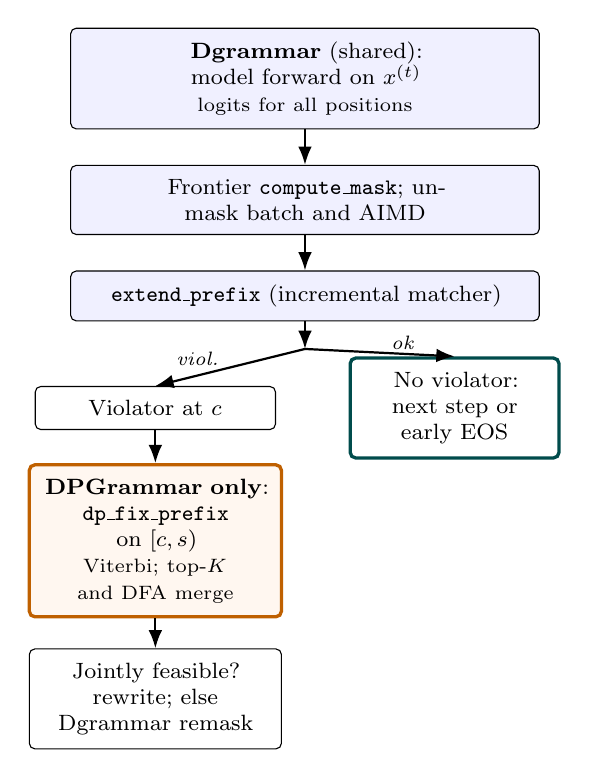
\begin{tikzpicture}[
  font=\footnotesize,
  >=Latex,
  proc/.style={draw, rounded corners=2pt, align=center, inner sep=5pt, fill=white},
  arr/.style={thick, ->},
  lbl/.style={inner sep=1pt, font=\scriptsize},
]
  % Shared Dgrammar steps (blue tint)
  \node[proc, fill=blue!6, text width=5.6cm] (fwd) at (0,0)
    {\textbf{Dgrammar} (shared): model forward on $x^{(t)}$\\
     {\scriptsize logits for all positions}};
  \node[proc, fill=blue!6, text width=5.6cm, below=0.45cm of fwd] (unm)
    {Frontier \texttt{compute\_mask}; unmask batch and AIMD};
  \node[proc, fill=blue!6, text width=5.6cm, below=0.45cm of unm] (chk)
    {\texttt{extend\_prefix} (incremental matcher)};
  % Fork point below chk
  \coordinate (split) at ($(chk.south)+(0,-0.35)$);
  % Left branch: violator path
  \node[proc, text width=2.7cm] (bad) at ($(split)+(-1.9,-0.75)$)
    {Violator at~$c$};
  \node[proc, text width=2.85cm, draw=orange!75!black, very thick, fill=orange!6,
        below=0.42cm of bad] (dp)
    {\textbf{DPGrammar only}:\\
     \texttt{dp\_fix\_prefix} on $[c,s)$\\
     {\scriptsize Viterbi; top-$K$ and DFA merge}};
  \node[proc, text width=2.85cm, below=0.38cm of dp] (fall)
    {Jointly feasible?\\rewrite; else Dgrammar remask};
  % Right branch: ok path
  \node[proc, draw=teal!60!black, very thick, text width=2.3cm]
        (ok) at ($(split)+(1.9,-0.75)$)
    {No violator:\\next step or\\early EOS};
  % Arrows
  \draw[arr] (fwd) -- (unm);
  \draw[arr] (unm) -- (chk);
  \draw[arr] (chk.south) -- (split);
  \draw[arr] (split) -- node[above left, lbl, pos=0.55] {\textit{viol.}} (bad.north);
  \draw[arr] (split) -- node[above right, lbl, pos=0.55] {\textit{ok}} (ok.north);
  \draw[arr] (bad) -- (dp);
  \draw[arr] (dp) -- (fall);
\end{tikzpicture}
\end{minipage}%
\hfill
% Right panel: token diagram
\begin{minipage}[c]{0.43\linewidth}
\centering
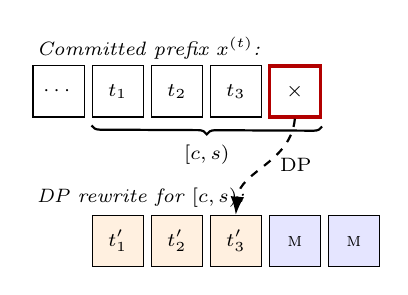
\begin{tikzpicture}[
  font=\footnotesize,
  >=Latex,
  tok/.style={draw, minimum width=6.5mm, minimum height=6.5mm,
              inner sep=0pt, align=center, font=\scriptsize},
]
  % ── Define all nodes first ──
  % Top row: committed prefix at y=0
  \node[tok] (p0) at (0.00, 0.00) {$\cdots$};
  \node[tok] (p1) at (0.75, 0.00) {$t_1$};
  \node[tok] (p2) at (1.50, 0.00) {$t_2$};
  \node[tok] (p3) at (2.25, 0.00) {$t_3$};
  \node[tok, draw=red!70!black, very thick] (pv) at (3.00, 0.00) {$\times$};
  % Bottom row: DP rewrite at y=-1.9
  \node[tok, fill=orange!12] (q1) at (0.75, -1.9) {$t_1'$};
  \node[tok, fill=orange!12] (q2) at (1.50, -1.9) {$t_2'$};
  \node[tok, fill=orange!12] (q3) at (2.25, -1.9) {$t_3'$};
  \node[tok, fill=blue!10]   (m1) at (3.00, -1.9) {\textsc{m}};
  \node[tok, fill=blue!10]   (m2) at (3.75, -1.9) {\textsc{m}};
  % ── Row labels (above each row) ──
  \node[anchor=west, font=\scriptsize\itshape] at (-0.40, 0.55)
    {Committed prefix $x^{(t)}$:};
  \node[anchor=west, font=\scriptsize\itshape] at (-0.40, -1.35)
    {DP rewrite for $[c,s)$:};
  % ── Brace on top row marking [c,s) ──
  \draw[decorate, decoration={brace, amplitude=3pt, mirror}, thick]
    ($(p1.south west)+(0,-0.10)$) --
    node[below=3pt, font=\scriptsize] {$[c,s)$}
    ($(pv.south east)+(0,-0.10)$);
  % ── DP correction arrow (violator → rewrite) ──
  \draw[dashed, ->, thick]
    (pv.south) to[out=-95, in=85]
    node[right, font=\scriptsize, pos=0.48, xshift=1pt] {DP}
    (q3.north);
\end{tikzpicture}
\end{minipage}
\caption{\label{fig:dp-denoise}%
  \textbf{Dgrammar} (blue tinted): one denoising step applies a full model
  forward, frontier masking and AIMD unmasking, and incremental
  \texttt{extend\_prefix}. \textbf{DPGrammar} (orange): when a violator is
  detected at position $c$, \texttt{dp\_fix\_prefix} jointly rewrites the span
  $[c,s)$ via Viterbi over top-$K$ tokens before falling back to greedy
  remasking.}
\end{figure*}

\subsection{Completion after generation}
Both systems share driver side repair after the diffusion phase: grammar guided greedy autocomplete, masked extension, grammar only closing, and minimal JSON synthesis from the schema when required.

\subsection{Implementation and compute}
Code builds on PyTorch, Transformers, \textsc{llguidance}, and the constrained diffusion CD4d style bindings; benchmarks run on \textbf{Modal} with NVIDIA \textbf{A100} GPUs in our experiments. Backbone is \textbf{GSAI ML LLaDA 8B Instruct}. Block length 32 for timed async runs, remasking \texttt{low\_confidence}, temperature 0.2 in the driver, seed 0 unless noted. Full hyperparameter tables can be folded into an appendix if space is tight.

\subsection{Experimental design and metrics}
\textbf{Schema validity} is the primary outcome (binary \texttt{valid} per instance). \textbf{Wall time} per instance measures end to end driver time. We report median, mean, and P95 to capture heavy tails (LAVE hits a 120\,s cap in our run; DPGrammar shows rare long runs). \textbf{Effective constraint \%} aggregates grammar check time, token selection, mask wait, and autocomplete mask time relative to forward plus overhead, as emitted by \texttt{run\_dgrammar\_timed.py}. \textbf{Resamples} counts remasking events. We did not compute formal confidence intervals; differences are large on validity, but future work should add bootstrap CIs on the same split.

\section{Results}
\label{sec:results}

%% ─── Figure: LAVE vs Dgrammar single denoising step ─────────────────────────
\begin{figure*}[t]
\centering
\begin{minipage}[t]{0.46\linewidth}
\centering
{\small\bfseries LAVE} {\small--- stochastic lookahead-then-verify}
\vspace{4pt}

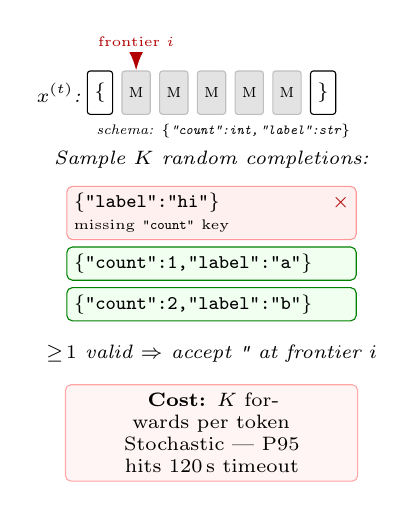
\begin{tikzpicture}[
  font=\footnotesize,>=Latex,
  tok/.style={draw,rounded corners=1pt,inner sep=2.5pt,minimum height=5.5mm,
              align=center,font=\scriptsize\ttfamily},
  mtok/.style={tok,fill=gray!22,draw=gray!50,font=\scriptsize},
  arr/.style={->,thick},
  samp/.style={draw,rounded corners=2pt,inner sep=2.5pt,font=\scriptsize,
               text width=3.5cm,align=left},
]
  \node[tok] (i0) at (0,0) {\{};
  \node[mtok,right=3pt of i0] (i1) {\textsc{m}};
  \node[mtok,right=3pt of i1] (i2) {\textsc{m}};
  \node[mtok,right=3pt of i2] (i3) {\textsc{m}};
  \node[mtok,right=3pt of i3] (i4) {\textsc{m}};
  \node[mtok,right=3pt of i4] (i5) {\textsc{m}};
  \node[tok,right=3pt of i5]  (i6) {\}};
  \node[font=\scriptsize\itshape,anchor=east] at (-0.12,0) {$x^{(t)}$:};
  \node[font=\tiny\itshape,anchor=west] at ($(i0.south west)+(0,-0.2)$)
    {schema: \texttt{\{"count":int,\,"label":str\}}};
  \draw[arr,red!70!black] (i1.north)++(0,.24) -- (i1.north);
  \node[font=\tiny,red!70!black,above=0.18cm of i1] {frontier $i$};

  \node[font=\scriptsize\itshape] (sl) at ($(i0)!0.5!(i6)+(0,-0.85)$)
    {Sample $K$ random completions:};
  \node[samp,fill=red!6,draw=red!40,anchor=north] (s1) at ($(sl.south)+(0,-0.1)$)
    {\texttt{\{"label":"hi"\}}\hfill\textcolor{red!70!black}{$\times$}\\
     {\tiny missing \texttt{"count"} key}};
  \node[samp,fill=green!6,draw=green!50!black,anchor=north] (s2) at ($(s1.south)+(0,-0.08)$)
    {\texttt{\{"count":1,"label":"a"\}}\hfill\textcolor{green!60!black}{$\checkmark$}};
  \node[samp,fill=green!6,draw=green!50!black,anchor=north] (s3) at ($(s2.south)+(0,-0.08)$)
    {\texttt{\{"count":2,"label":"b"\}}\hfill\textcolor{green!60!black}{$\checkmark$}};

  \node[font=\scriptsize\itshape,anchor=north] (dec) at ($(s3.south)+(0,-0.18)$)
    {$\geq\!1$ valid $\Rightarrow$ accept \texttt{"} at frontier $i$};
  \node[draw=red!35,fill=red!4,rounded corners=2pt,font=\scriptsize,
        text width=3.5cm,align=center,inner sep=3pt,anchor=north]
    at ($(dec.south)+(0,-0.15)$)
    {\textbf{Cost:} $K$ forwards per token\\Stochastic — P95 hits 120\,s timeout};
\end{tikzpicture}
\end{minipage}%
\hfill
\begin{minipage}[t]{0.46\linewidth}
\centering
{\small\bfseries Dgrammar} {\small--- deterministic frontier masking}
\vspace{4pt}

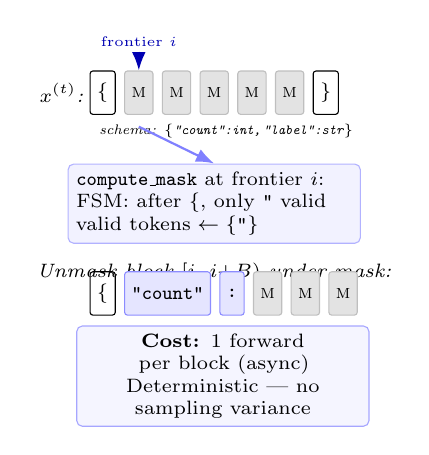
\begin{tikzpicture}[
  font=\footnotesize,>=Latex,
  tok/.style={draw,rounded corners=1pt,inner sep=2.5pt,minimum height=5.5mm,
              align=center,font=\scriptsize\ttfamily},
  mtok/.style={tok,fill=gray!22,draw=gray!50,font=\scriptsize},
  ctok/.style={tok,fill=blue!10,draw=blue!45},
  arr/.style={->,thick},
]
  \node[tok] (i0) at (0,0) {\{};
  \node[mtok,right=3pt of i0] (i1) {\textsc{m}};
  \node[mtok,right=3pt of i1] (i2) {\textsc{m}};
  \node[mtok,right=3pt of i2] (i3) {\textsc{m}};
  \node[mtok,right=3pt of i3] (i4) {\textsc{m}};
  \node[mtok,right=3pt of i4] (i5) {\textsc{m}};
  \node[tok,right=3pt of i5]  (i6) {\}};
  \node[font=\scriptsize\itshape,anchor=east] at (-0.12,0) {$x^{(t)}$:};
  \node[font=\tiny\itshape,anchor=west] at ($(i0.south west)+(0,-0.2)$)
    {schema: \texttt{\{"count":int,\,"label":str\}}};
  \draw[arr,blue!70!black] (i1.north)++(0,.24) -- (i1.north);
  \node[font=\tiny,blue!70!black,above=0.18cm of i1] {frontier $i$};

  \node[draw=blue!30,fill=blue!5,rounded corners=2pt,font=\scriptsize,
        text width=3.5cm,inner sep=3pt,anchor=north] (mask)
    at ($(i0)!0.5!(i6)+(0,-0.9)$)
    {\texttt{compute\_mask} at frontier $i$:\\
     FSM: after \texttt{\{}, only \texttt{"} valid\\
     $\mathrm{valid\ tokens} \gets \{\texttt{"}\}$};
  \draw[arr,blue!50] ($(i1.south)+(0,-0.15)$) -- (mask.north);

  \node[font=\scriptsize\itshape,anchor=north] (ul) at ($(mask.south)+(0,-0.12)$)
    {Unmask block $[i,\,i{+}B)$ under mask:};

  \node[tok]  (c0) at (0,-2.55) {\{};
  \node[ctok,right=3pt of c0] (c1) {"count"};
  \node[ctok,right=3pt of c1] (c2) {:};
  \node[mtok,right=3pt of c2] (c3) {\textsc{m}};
  \node[mtok,right=3pt of c3] (c4) {\textsc{m}};
  \node[mtok,right=3pt of c4] (c5) {\textsc{m}};
  \node[font=\tiny\itshape,blue!60!black,anchor=north]
    at ($(c1)!0.5!(c2)+(0,-0.3)$) {committed under grammar};

  \node[draw=blue!35,fill=blue!4,rounded corners=2pt,font=\scriptsize,
        text width=3.5cm,align=center,inner sep=3pt]
    at ($(c0)!0.5!(c5)+(0,-1.05)$)
    {\textbf{Cost:} 1 forward per block (async)\\Deterministic — no sampling variance};
\end{tikzpicture}
\end{minipage}
\caption{\label{fig:denoise-compare}%
  One denoising step under schema \texttt{\{"count":int,\,"label":str\}}.
  \textbf{LAVE} \citep{zhang2026lookaheadthenverifyreliableconstraineddecoding}
  (left) samples $K$ random completions at each frontier token, accepting it
  only when $\geq\!1$ suffix is valid—stochastic and $K\!\times$ more expensive
  per token, hitting the 120\,s per-instance timeout on hard schemas.
  \textbf{Dgrammar} (right) runs \texttt{compute\_mask} on the incremental FSM
  state and unmasks an entire block under that mask in one forward pass,
  overlapped with the next mask computation; the result is deterministic.}
\end{figure*}

Table~\ref{tab:main} reports aggregate metrics. LAVE reaches 68.8\% validity on $n{=}586$ (nine shards) with median wall time 28.45\,s and P95 78.32\,s. Dgrammar reaches 84.9\% on $n{=}511$ with median 10.23\,s and median effective constraint 20.43\%. DPGrammar reaches 99.2\% validity on the same 511 instances, median 12.87\,s, mean resamples 1.06 versus 32.43 for Dgrammar.

\paragraph{Qualitative observations.}
Instances where LAVE approaches the timeout often correspond to hard schemas or long generations; Dgrammar avoids sampling variance but can require many greedy resamples when joint structure is wrong, which DPGrammar mitigates. Error modes for DPGrammar on remaining failures include completion phase limits and schemas where minimal JSON fallback is brittle; we leave detailed case studies to appendix space.

\begin{table*}[t]
\centering
\small
\begin{tabular}{lcccccc}
\toprule
\textbf{Method} &
  \textbf{Validity} &
  \textbf{Med.\ time (s)} &
  \textbf{Mean time (s)} &
  \textbf{P95 time (s)} &
  \textbf{Med.\ eff.\ const.\ \%} &
  \textbf{Mean resamples} \\
\midrule
LAVE\,$^\ddagger$ {\scriptsize(reimpl., $n{=}586$)}
  & 68.8\%        & 28.45 & 34.59          & 78.32  & ---           & 222.6\,$^\S$ \\
Dgrammar {\scriptsize(async, $n{=}511$)}
  & 84.9\%        & 10.23 & 13.14          & 32.10  & 20.43         & 32.43 \\
DPGrammar {\scriptsize(\texttt{dp}, $n{=}511$)}
  & \textbf{99.2\%} & 12.87 & 14.96          & 28.55 & \textbf{1.22} & \textbf{1.06} \\
\bottomrule
\end{tabular}
\caption{\label{tab:main}%
  \texttt{jsb\_medium} results (seed 0, $T{=}128$ steps).
  Dgrammar and DPGrammar are evaluated on the same 511 instances
  (nine-shard protocol); DPGrammar adds \texttt{dp\_fix\_prefix} on top.
  LAVE \citep{zhang2026lookaheadthenverifyreliableconstraineddecoding}
  uses a nine-shard split covering 586 instances.}
\end{table*}

\noindent$^\ddagger$ LAVE nine-shard evaluation ($n{=}586$); median and P95 reflect sampling based verification cost.\\
\noindent$^\S$ LAVE resamples count lookahead verification draws, not token re-generations; the concept differs from Dgrammar/DPGrammar resamples.

%% ─── Figure: Why DP boosts validity ─────────────────────────────────────────
\begin{figure*}[t]
\centering
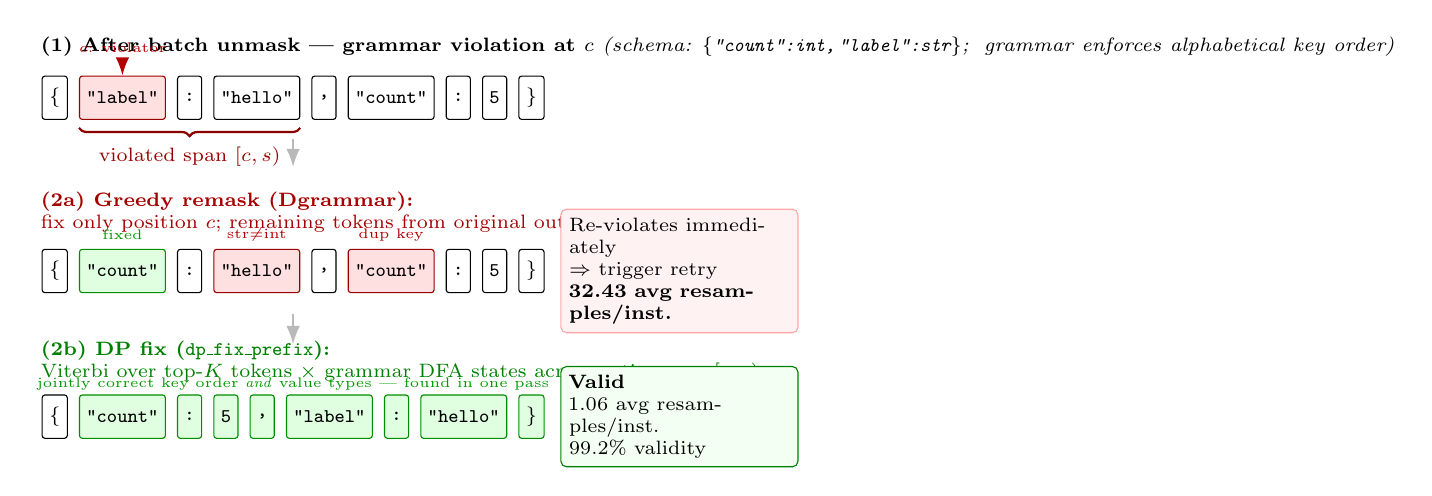
\begin{tikzpicture}[
  font=\footnotesize,>=Latex,
  tok/.style={draw,rounded corners=1pt,inner sep=2.5pt,minimum height=5.5mm,
              align=center,font=\scriptsize\ttfamily},
  ntok/.style={tok},
  btok/.style={tok,fill=red!12,draw=red!60!black},
  vtok/.style={tok,fill=green!12,draw=green!55!black},
  arr/.style={->,thick},
]

%% ── (1) Violated block ───────────────────────────────────────────────────────
\node[font=\scriptsize\bfseries,anchor=west,align=left]
  at (-0.3,0.65)
  {(1)~After batch unmask — grammar violation at $c$
   {\normalfont\itshape
    (schema: \texttt{\{"count":int,\,"label":str\}};\;
    grammar enforces alphabetical key order)}};

\node[ntok] (a0) at (0,0) {\{};
\node[btok,right=4pt of a0] (a1) {"label"};
\node[ntok,right=4pt of a1] (a2) {:};
\node[ntok,right=4pt of a2] (a3) {"hello"};
\node[ntok,right=4pt of a3] (a4) {,};
\node[ntok,right=4pt of a4] (a5) {"count"};
\node[ntok,right=4pt of a5] (a6) {:};
\node[ntok,right=4pt of a6] (a7) {5};
\node[ntok,right=4pt of a7] (a8) {\}};

\draw[arr,red!70!black] (a1.north)++(0,.22) -- (a1.north);
\node[font=\tiny,red!70!black] at ($(a1.north)+(0,.35)$) {$c$: violator};

\draw[decorate,decoration={brace,amplitude=3pt,mirror},thick,red!55!black]
  ($(a1.south west)+(0,-0.1)$) --
  node[below=3pt,font=\scriptsize,red!60!black] {violated span $[c,s)$}
  ($(a3.south east)+(0,-0.1)$);

%% ── Arrow down ───────────────────────────────────────────────────────────────
\draw[arr,gray!55] ($(a0)!0.5!(a8)+(0,-0.52)$) -- ++(0,-0.36);

%% ── (2a) Greedy remask (Dgrammar) ────────────────────────────────────────────
\node[font=\scriptsize\bfseries,anchor=west,red!65!black,align=left]
  at (-0.3,-1.45)
  {(2a)~Greedy remask (Dgrammar):\\
   \normalfont fix only position $c$; remaining tokens from original output are unchanged};

\node[ntok] (b0) at (0,-2.2) {\{};
\node[vtok,right=4pt of b0] (b1) {"count"};
\node[ntok,right=4pt of b1] (b2) {:};
\node[btok,right=4pt of b2] (b3) {"hello"};
\node[ntok,right=4pt of b3] (b4) {,};
\node[btok,right=4pt of b4] (b5) {"count"};
\node[ntok,right=4pt of b5] (b6) {:};
\node[ntok,right=4pt of b6] (b7) {5};
\node[ntok,right=4pt of b7] (b8) {\}};

\node[font=\tiny,green!60!black] at ($(b1.north)+(0,.18)$) {fixed};
\node[font=\tiny,red!70!black]   at ($(b3.north)+(0,.18)$) {str$\neq$int};
\node[font=\tiny,red!70!black]   at ($(b5.north)+(0,.18)$) {dup key};

\node[draw=red!35,fill=red!5,rounded corners=2pt,font=\scriptsize,
      text width=2.8cm,align=left,inner sep=3pt,anchor=west]
  at ($(b8.east)+(0.2,0)$)
  {Re-violates immediately\\$\Rightarrow$ trigger retry\\
   \textbf{32.43 avg resamples/inst.}};

%% ── Arrow down ───────────────────────────────────────────────────────────────
\draw[arr,gray!55] ($(b0)!0.5!(b8)+(0,-0.55)$) -- ++(0,-0.38);

%% ── (2b) DP fix (DPGrammar) ──────────────────────────────────────────────────
\node[font=\scriptsize\bfseries,anchor=west,green!50!black,align=left]
  at (-0.3,-3.35)
  {(2b)~DP fix (\texttt{dp\_fix\_prefix}):\\
   \normalfont
   Viterbi over top-$K$ tokens $\times$ grammar DFA states across entire span $[c,s)$};

\node[ntok] (d0) at (0,-4.05) {\{};
\node[vtok,right=4pt of d0] (d1) {"count"};
\node[vtok,right=4pt of d1] (d2) {:};
\node[vtok,right=4pt of d2] (d3) {5};
\node[vtok,right=4pt of d3] (d4) {,};
\node[vtok,right=4pt of d4] (d5) {"label"};
\node[vtok,right=4pt of d5] (d6) {:};
\node[vtok,right=4pt of d6] (d7) {"hello"};
\node[vtok,right=4pt of d7] (d8) {\}};

\node[font=\tiny,green!60!black] at ($(d1)!0.5!(d7)+(0,.42)$)
  {jointly correct key order \emph{and} value types — found in one pass};

\node[draw=green!50!black,fill=green!5,rounded corners=2pt,font=\scriptsize,
      text width=2.8cm,align=left,inner sep=3pt,anchor=west]
  at ($(d8.east)+(0.2,0)$)
  {\textbf{Valid} $\checkmark$\\
   1.06 avg resamples/inst.\\
   99.2\% validity};
\end{tikzpicture}
\caption{\label{fig:dp-validity-boost}%
  Why DPGrammar lifts validity from 84.9\,\% (Dgrammar) to 99.2\,\%.
  \textbf{(1)}~A batch unmask produces \texttt{"label"} before \texttt{"count"},
  violating the grammar's alphabetical key-order constraint; the violator at
  position $c$ spans $[c,s)$.
  \textbf{(2a)}~Dgrammar's greedy remask corrects only $c$: the grammar mask
  forces \texttt{"count"} there, but the value slot still holds
  \texttt{"hello"} (a string in an integer field) and the original
  \texttt{"count"} key remains as a duplicate—causing immediate re-violation
  and an average of 32.43 resamples per instance (LAVE: 222.6 lookahead
  draws with similar failure modes on hard schemas).
  \textbf{(2b)}~\texttt{dp\_fix\_prefix} runs Viterbi over top-$K$ token
  candidates across every position in $[c,s)$ simultaneously, jointly
  finding \texttt{"count":5,"label":"hello"}—correct order, correct types,
  no duplicates—in one pass, reducing to 1.06 avg resamples and 99.2\%
  validity.}
\end{figure*}

\section{Discussion}

\paragraph{Interpretation.}
The gap between LAVE and Dgrammar supports the claim that deterministic frontier parsing with incremental masks is a strong fit for schema constrained JSON under diffusion when sampling based verification is costly or brittle. The gap between Dgrammar and DPGrammar on the same instances isolates the value of joint segment repair beyond greedy remasking.

\paragraph{Strengths.}
DPGrammar achieves the highest validity and lowest resample churn in our table; Dgrammar offers a simpler system with strong validity gains over LAVE and competitive medians.

\paragraph{Weaknesses and surprises.}
Effective constraint \% definitions differ in interpretability across methods; DPGrammar's median is low partly because fewer retries occur. Mean and median wall times are close for DPGrammar in our run. DPGrammar validity is below 100\%, so completion and fallback stages still matter.

\paragraph{Implications.}
Practitioners should report forward versus constraint splits, not only total time. For research, joint repair on violation segments is a lightweight add on relative to full sequence DP \citep{suresh2025dingoconstrainedinferencediffusion}.

\section{Conclusion and Future Work}

We studied grammar constrained decoding for dLLMs with \textbf{Dgrammar}, a frontier incremental system engineered for deterministic alignment and timing visibility, and \textbf{DPGrammar}, which adds segment level Viterbi repair. On \texttt{jsb\_medium}, Dgrammar improves substantially over a reproduced LAVE baseline; DPGrammar improves further over Dgrammar on matched instances. \textbf{Broader takeaway:} structured generation with diffusion needs both algorithmic ideas and systems style measurement; parser grounded frontiers and joint repair are practical levers.

\textbf{Future work} includes evaluating LAVE on the same nine shard split for a strictly controlled three way comparison; extending to additional JSON splits or code grammars; bootstrap confidence intervals; and exploring tighter integration with sparse automata acceleration \citep{su2026vectorizingtrieefficientconstrained} for very large vocabularies.

\section{Limitations}

LAVE and our methods are not evaluated on identical instance sets in Table~\ref{tab:main}, so cross column comparisons involving LAVE are indicative rather than strictly controlled. The validity flag depends on benchmark extraction; functional tests beyond schema syntax are not central here. Hyperparameter tuning was limited; different $T$, block sizes, or temperature could shift outcomes. DPGrammar explores top $K$ tokens per DP position, which can miss globally optimal tokens outside the top $K$. Compute was cloud A100; other hardware changes overlap benefits.

\section{Ethical Considerations}

Structured generation can reduce malformed outputs in downstream automation, but \emph{valid JSON is not always semantically safe or fair}: schemas can encode biased or incomplete coverage of user intent. Models and grammars should be reviewed for misuse in high stakes settings (medical, financial). Our benchmark instances originate from public style schema tasks; they may not represent all languages or cultures. Researchers and deployers should combine syntactic guarantees with content moderation and policy controls. We use open backbone weights and public style evaluation data; users of our code should respect model licenses and avoid deploying unreviewed systems in sensitive domains without human oversight.


\bibliography{custom}


% --- APPENDIX ---
% \appendix

\section{DPGrammar Algorithm (\texttt{dp\_fix\_prefix})}
\label{app:alg}

Algorithm~\ref{alg:dpgrammar} gives the full pseudocode for the Viterbi segment repair used by DPGrammar.
Given a violated span $[c,s)$ detected during generation, the algorithm maintains a dictionary of live DFA states, each mapped to its highest-scoring path (matcher clone and cumulative log-probability).
At each position it probes the top-$K$ vocabulary entries via rollback—no cloning—and records the best (prev\_state, token) pair for each reachable DFA state (Viterbi merge).
After the loop, it clones one matcher per surviving state (Phase~2) and records the backtrack pointers.
Backtracking from the best final state yields the minimal set of token replacements needed to make the span grammar-valid.

Two design choices keep the algorithm efficient.
First, DFA states are identified by \texttt{bytes(matcher.compute\_logit\_bias())}, a compact proxy for the automaton node; this bounds the number of active states by the grammar's DFA size ($\sim$20--200 for typical JSON schemas) rather than by $K^{\text{depth}}$.
Second, matcher clones are created only once per surviving state per step (Phase~2), not once per (state, candidate) pair; cloning cost is therefore $O(|\text{winners}|) \leq O(\text{DFA size})$ per position rather than $O(K \times |\text{states}|)$.

The span $[c,s)$ is bounded by \texttt{find\_constraint\_end}, which probes forward from $c$ using the grammar automaton and tracks bracket depth in the original token sequence to avoid stopping inside an unclosed array or object.
The DP is thus applied to a narrow window around the violated constraint rather than the full remaining sequence.

\IfFileExists{algpseudocode.sty}{
\begin{algorithm*}[t]
\caption{DPGrammar: Viterbi segment repair over a violated span (\texttt{dp\_fix\_prefix})}
\label{alg:dpgrammar}
\begin{algorithmic}[1]
\Require Violated span $[c,s)$; log-probabilities $\ell \in \mathbb{R}^{L \times |V|}$ from the current forward; grammar matcher $\mathcal{M}$ at the DFA state just before $c$; beam width $K$
\Ensure Replacement pairs $\{(p_i, t_i)\}$ maximising $\sum \log p(t_i)$ subject to grammar, or \textsc{Fail}
\State $P \gets [c,\, c{+}1,\, \ldots,\, s{-}1]$
\State $\mathit{states} \gets \{\operatorname{key}(\mathcal{M}) \mapsto (\mathcal{M},\ 0)\}$ \Comment{DFA-state $\to$ (matcher, cumulative log-prob)}
\State $\mathit{back} \gets \{\}$ \Comment{backtrack table}
\For{$i \gets 0$ \textbf{to} $|P|-1$}
    \State $T_K \gets \operatorname{top\text{-}K}(\ell[P[i]],\; k{=}K)$
    \State $\mathit{winners} \gets \{\}$
    \For{\textbf{each} $(\text{prev\_key},\, (\mathcal{M}_p,\, \sigma_p))$ \textbf{in} $\mathit{states}$}
        \For{\textbf{each} $(t,\, \ell_t)$ \textbf{in} $T_K$}
            \If{$\mathcal{M}_p.\operatorname{try\_consume}([t]) < 1$}
                \State $\mathcal{M}_p.\operatorname{rollback}(0)$; \textbf{continue}
            \EndIf
            \State $\sigma' \gets \sigma_p + \ell_t$;\quad $k' \gets \operatorname{key}(\mathcal{M}_p)$
            \State $\mathcal{M}_p.\operatorname{rollback}(1)$
            \If{$k' \notin \mathit{winners}$ \textbf{or} $\mathit{winners}[k'].\sigma < \sigma'$}
                \State $\mathit{winners}[k'] \gets (\text{prev\_key},\; t,\; \sigma')$ \Comment{Viterbi merge}
            \EndIf
        \EndFor
    \EndFor
    \If{$\mathit{winners} = \emptyset$}\ \Return \textsc{Fail} \EndIf
    \State $\mathit{next} \gets \{\}$
    \For{\textbf{each} $(k',\, (\text{prev\_key},\, t,\, \sigma'))$ \textbf{in} $\mathit{winners}$} \Comment{Phase 2: clone once per surviving state}
        \State $\mathcal{M}' \gets \mathit{states}[\text{prev\_key}].\mathcal{M}.\operatorname{deep\_copy}()$;\quad $\mathcal{M}'.\operatorname{try\_consume}([t])$
        \State $\mathit{next}[k'] \gets (\mathcal{M}',\; \sigma')$;\quad $\mathit{back}[(i,\,k')] \gets (\text{prev\_key},\; t)$
    \EndFor
    \State $\mathit{states} \gets \mathit{next}$
\EndFor
\State $k^* \gets \arg\max_k\; \mathit{states}[k].\sigma$;\quad $\mathit{fixes} \gets []$;\quad $\text{cur} \gets k^*$
\For{$i \gets |P|-1$ \textbf{downto} $0$}
    \State $(\text{prev},\; t) \gets \mathit{back}[(i,\;\text{cur})]$
    \If{$t \neq x[P[i]]$}\ $\mathit{fixes}.\operatorname{append}(P[i],\; t)$ \EndIf
    \State $\text{cur} \gets \text{prev}$
\EndFor
\State \Return $\operatorname{reverse}(\mathit{fixes})$
\end{algorithmic}
\end{algorithm*}
}{}

\section{Case Study: Instance \texttt{o12610}}
\label{app:case}

We examine instance \texttt{o12610} from \texttt{jsb\_medium}, a representative case where LAVE completely fails while DPGrammar produces a clean, fully valid output in a single pass with zero resamples.

\paragraph{Schema.}
The schema describes a physical Wi-Fi radio device configuration (OpenWRT/LuCI format).
The critical constraints are enum fields on \texttt{htmode} and \texttt{hwmode}:

\begin{lstlisting}[style=appendixcode]
"htmode": { "type": "string",
  "enum": [null, "HT20", "HT40+", "HT40-",
           "VHT20", "VHT40", "VHT80"] },
"hwmode": { "type": "string",
  "enum": ["11b", "11g", "11a"] }
\end{lstlisting}

Additional fields include \texttt{channel} (\texttt{integer}, range 1--165), \texttt{id} (string), \texttt{short\_gi\_20/40/80} (boolean), and \texttt{rx\_stbc}/\texttt{tx\_stbc} (integer, 0--1).

\paragraph{Why LAVE fails (timeout, 120\,s, no output).}
LAVE's stochastic lookahead commits a token only if all $K$ randomly sampled completions yield a grammar-valid continuation.
For enum fields, this requires a random completion to land on exactly one of a small set of technical strings (e.g.\ \texttt{"VHT20"}, \texttt{"11a"}) drawn from a natural-language vocabulary.
The probability is near zero: LLaDA-8B assigns negligible probability mass to \texttt{"VHT20"} or \texttt{"HT40-"} as free continuations, so every lookahead batch fails the grammar check.
LAVE cannot commit even the first enum-constrained token and times out after 120\,s without producing any output.

\paragraph{DPGrammar (valid, 0 resamples, 6.7\,s).}
Frontier masking restricts the vocabulary at each position to the set of tokens permitted by the grammar automaton.
For the \texttt{htmode} field, only the four tokens spelling out a valid enum value are unmasked; the model samples from this constrained set directly.
Because the automaton guides every token choice, no violation occurs and the Viterbi DP is never triggered (0 resample events, 0 DP calls).
The output is complete and semantically coherent:

\begin{lstlisting}[style=appendixcode]
{
    "channel": 60,
    "htmode": "VHT20",
    "hwmode": "11a",
    "id": "pci-wifi-1",
    "rx_stbc": 1,
    "short_gi_20": true,
    "short_gi_40": true,
    "short_gi_80": false,
    "tx_stbc": 1
}
\end{lstlisting}

All enum constraints are satisfied (\texttt{htmode} $\in$ allowed set, \texttt{hwmode} $=$ \texttt{"11a"}), the channel is within range, and boolean/integer fields are correctly typed.
Total wall time is 6.7\,s versus LAVE's 120\,s timeout—an 18$\times$ speedup on this instance.

\paragraph{Summary.}
This instance illustrates the general failure mode of stochastic lookahead on enum-constrained fields: the probability of a random natural-language completion matching a specific technical string (e.g.\ \texttt{"VHT20"}) is effectively zero, so LAVE never commits.
Frontier masking (shared by Dgrammar and DPGrammar) sidesteps this entirely by restricting the model's sampling distribution to the valid set at each position.
On instances where frontier masking prevents all violations, DPGrammar's Viterbi repair is never invoked—the method degrades gracefully to pure frontier-masked generation at the speed of a single unconstrained diffusion pass.

\section{Hyperparameters}
\label{app:hyperparams}

All experiments use LLaDA-8B-Instruct as the backbone, run on Modal with NVIDIA A100 GPUs.
Table~\ref{tab:hyperparams} lists the shared settings across all three methods.

\begin{table}[h]
\centering
\small
\begin{tabular}{ll}
\toprule
\textbf{Hyperparameter} & \textbf{Value} \\
\midrule
Diffusion steps $T$          & 128 \\
Random seed                  & 0 \\
Block length                 & 32 \\
Remasking strategy           & Low-confidence \\
Temperature                  & 0.2 \\
Top-$K$ (DPGrammar DP)       & 100 \\
Max resample attempts        & 500 (LAVE), 200 (ours) \\
Timeout threshold            & 120\,s \\
\bottomrule
\end{tabular}
\caption{Shared hyperparameters for all benchmark runs on \texttt{jsb\_medium}.}
\label{tab:hyperparams}
\end{table}

\section{Dataset and Instance Filtering}
\label{app:data}

We evaluate on the \texttt{Github\_medium} split of JSONSchemaBench, which contains 586 instances.
Of these, 75 are excluded from all comparisons because \textsc{llguidance} rejects their schemas at compile time: LAVE immediately returns \texttt{valid=false} with the error \texttt{"Prompt does not conform to grammar"}; Dgrammar and DPGrammar silently skip them via the same \textsc{llguidance} guard.
Since all three methods behave identically on these 75 instances, including them would inflate LAVE's failure count without providing a meaningful comparison.
All results in Table~\ref{tab:main} are therefore reported on the matched $n{=}511$ subset.

\section{Timing Breakdown}
\label{app:timing}

Table~\ref{tab:timing} reports per-method timing statistics supplementing Table~\ref{tab:main}.
Forward time dominates in all cases; constraint overhead is a small fraction for Dgrammar and DPGrammar.
LAVE's higher mean time is driven by timeout instances (capped at 120\,s); its median is lower because the majority of instances either succeed quickly or exhaust their resample budget early.
Effective constraint time for DPGrammar is near zero on instances where no DP repair is triggered; the non-trivial mean reflects the small fraction of instances that require one or more Viterbi passes.

\begin{table*}[h]
\centering
\small
\begin{tabular}{lrrr}
\toprule
\textbf{Metric} & \textbf{LAVE} & \textbf{Dgrammar} & \textbf{DPGrammar} \\
\midrule
Avg fwd passes              & 99.2  & 104.7 & 99.4  \\
Constraint overhead (\%)    & 11.95 & 24.25 & 12.67 \\
Eff.\ constraint (\%)       & —     & 20.43 & 1.22  \\
Per-token total (ms)        & 111.5 & 100.7 & 71.9  \\
Per-token constraint (ms)   & 6.64  & 8.26  & 0.30  \\
Avg mask compute (ms)       & —     & 427.2 & 577.0 \\
Avg forward total (ms)      & 3951  & 4612  & 4229  \\
\bottomrule
\end{tabular}
\caption{Detailed timing breakdown on \texttt{jsb\_medium} ($n{=}511$ matched instances).
Effective constraint \% measures time spent in grammar-check calls that were on the critical path; it is not available for LAVE, which lacks the same instrumentation.}
\label{tab:timing}
\end{table*}


\end{document}
